\subsection{Entwicklung der Benutzeroberfläche}
\label{subsec:entwicklung-der-benutzeroberflache}

Die Benutzeroberfläche wurde in HTML, CSS und JavaScript unter Verwendung der Jinja2-Template-Engine realisiert.

Alle relevanten Dateien für die Darstellung der Seiten befinden sich in den Ordnern \code{static} und \code{templates}.

Der Ordner \code{templates} enthält alle relevanten Jinja2-Templates bzw. HTML-Dateien.
Hierbei dient das HTML-Dokument \code{base.html} als das Grundgerüst für drei verschiedene Seiten.
Es beinhaltet die Elemente den Navigator zum Wechsel zwischen den Seiten, die Überschrift und das Messagefeld für Fehler und Systemnachrichten, die auf allen drei Seiten vorkommen.
Außerdem enthält es die Verknüpfung zu den CSS-Dateien \code{bootstrap.min.css} und \code{style.css} in \code{static}, die im Unterordner \code{css} liegen.
Sie verändert das Aussehen der Benutzeroberfläche, um ein abgerundetes Design zu erhalten.

Die drei anderen HTML-Dateien \code{upload.html}, \code{reports.html} und \code{dut\_analyse.html} werden durch Jinja2 in \code{base.html} eingebunden, um so folgende drei Seiten zu erstellen:

1. XML hochladen (\code{upload.html}): Hochladen und Einlesen von XML-Dateien.
Die Seite ist in der folgenden Abbildung \ref{fig: Webseite für XML hochladen} dargestellt.

\begin{figure}[H]
    \centering
    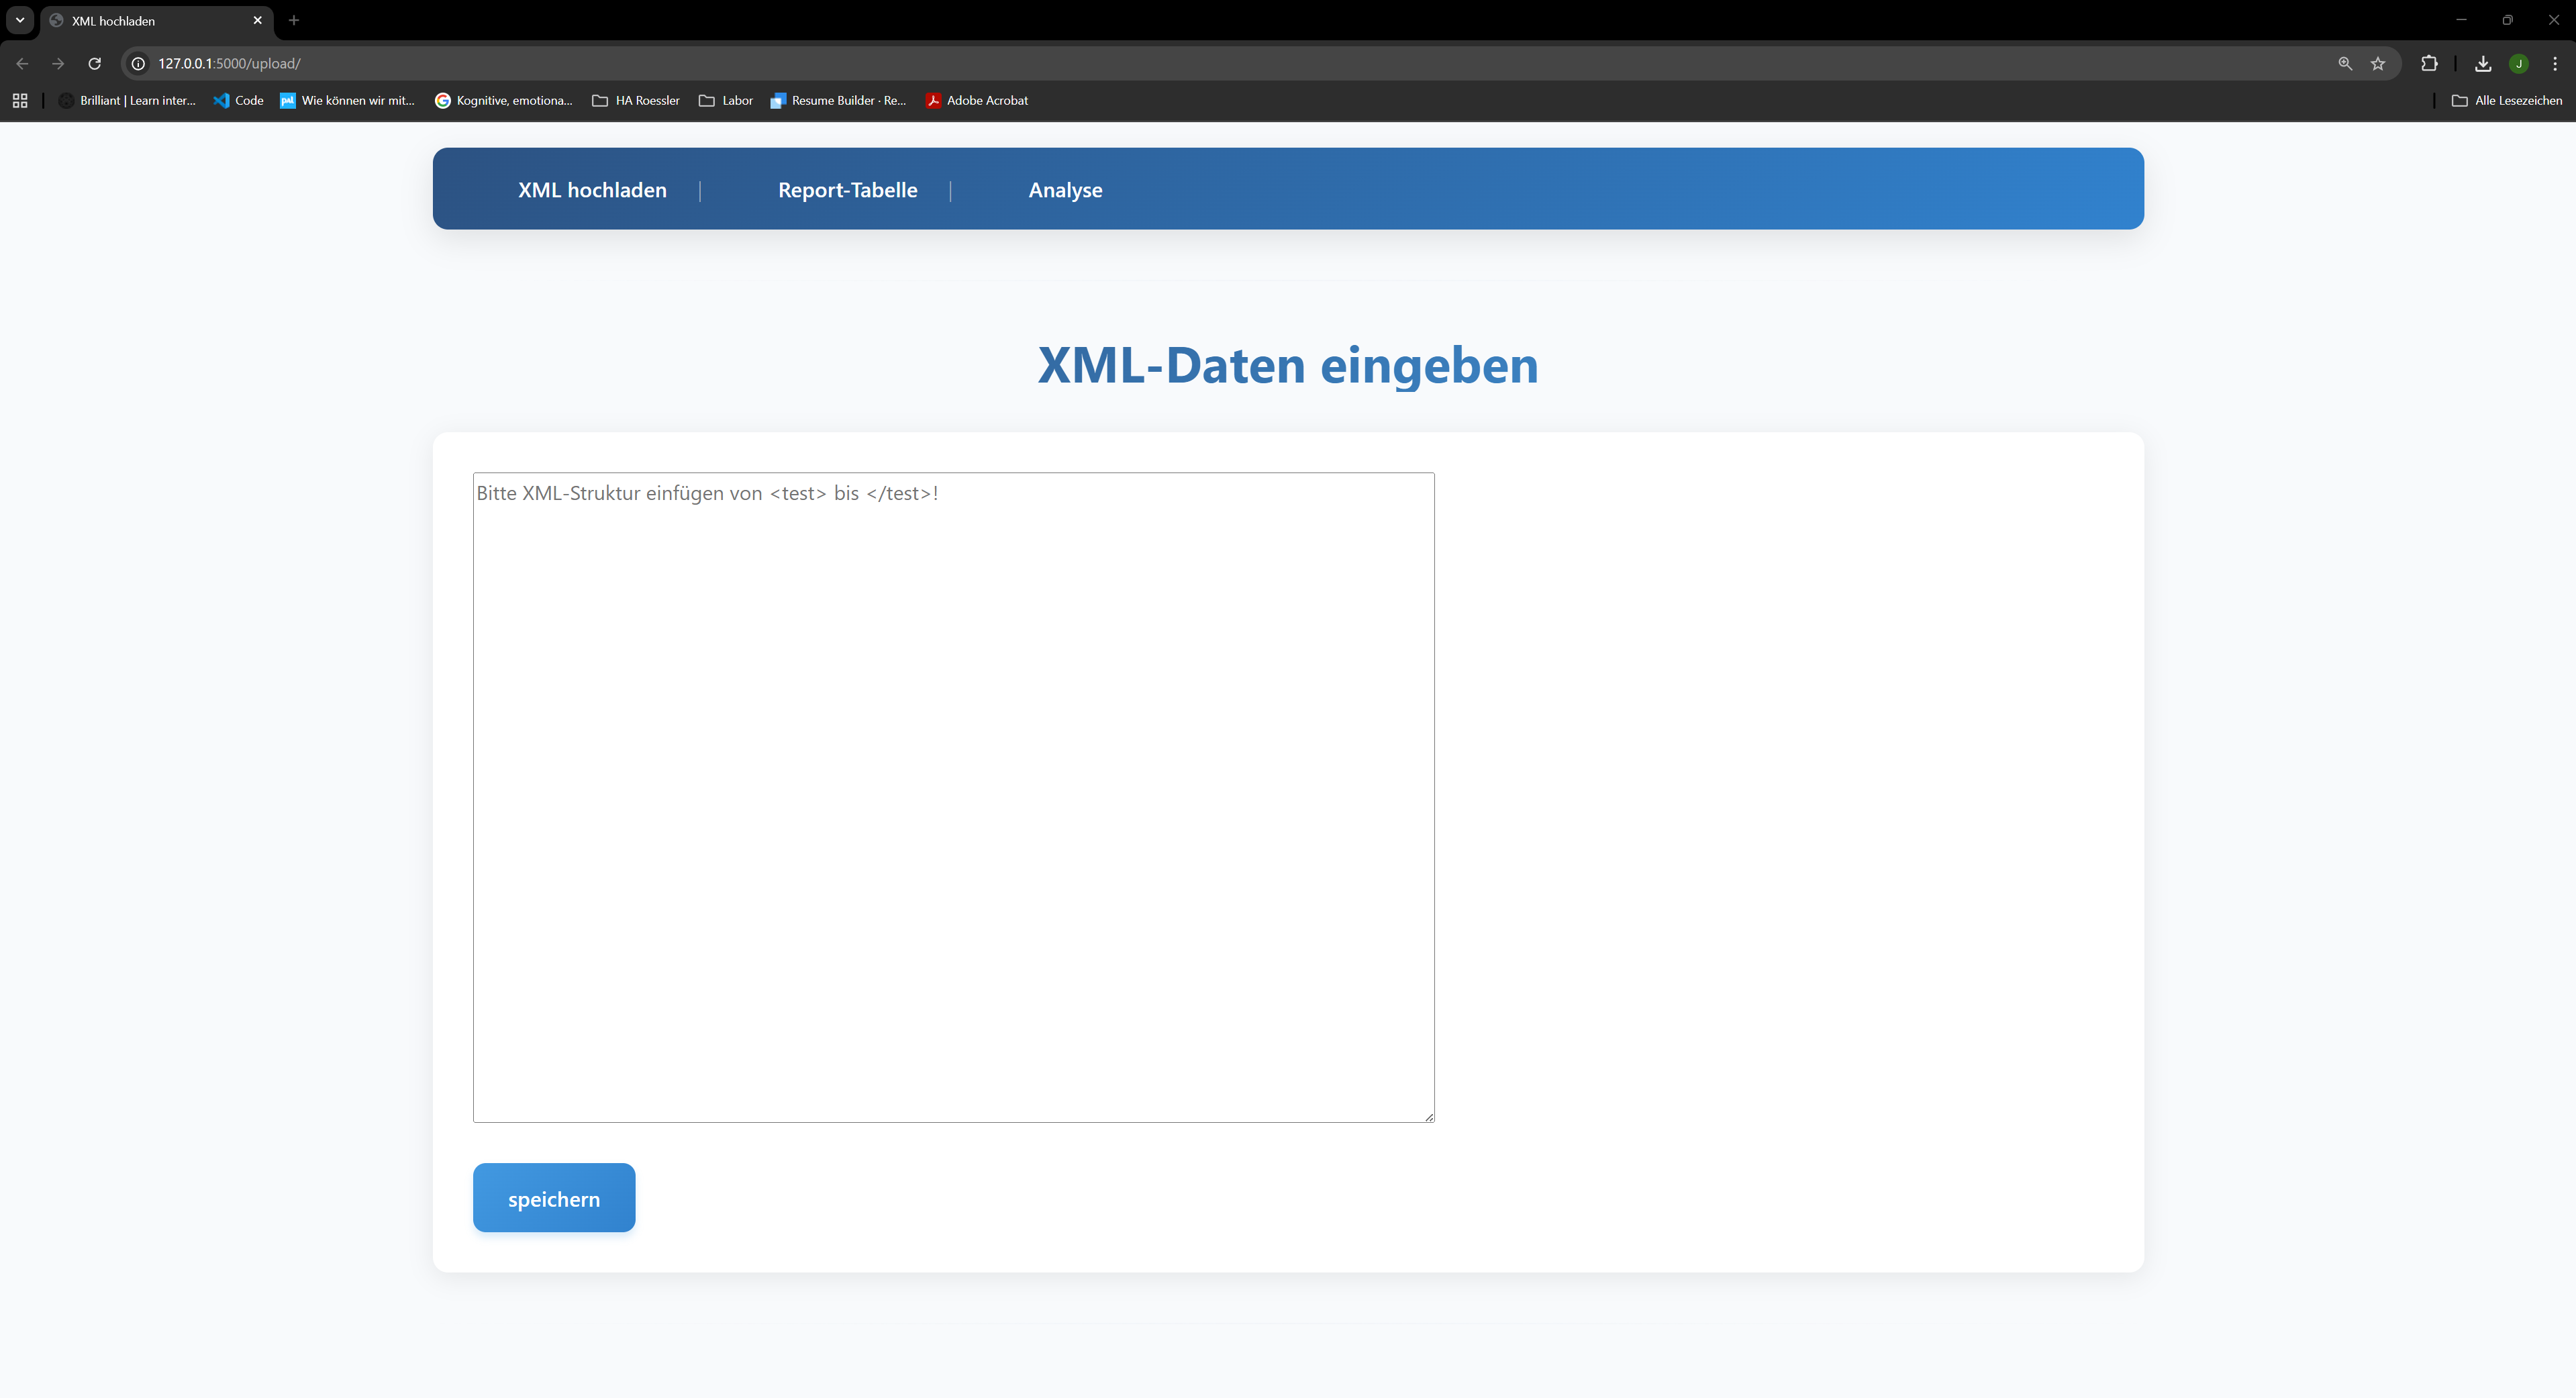
\includegraphics[width=1\textwidth]{Grafiken/Bild XML hochladen}
    \caption{Erstellte Webseite für XML hochladen in Browserfenster}
    \label{fig: Webseite für XML hochladen}
    {Quelle: Eigene Darstellung}
\end{figure}

2. Report-Tabelle (\code{reports.html}): Übersicht aller eingelesenen Testberichte in einer Tabelle.
Die Seite ist in der folgenden Abbildung \ref{fig: Webseite für Report-Tabelle} dargestellt.

\begin{figure}[H]
    \centering
    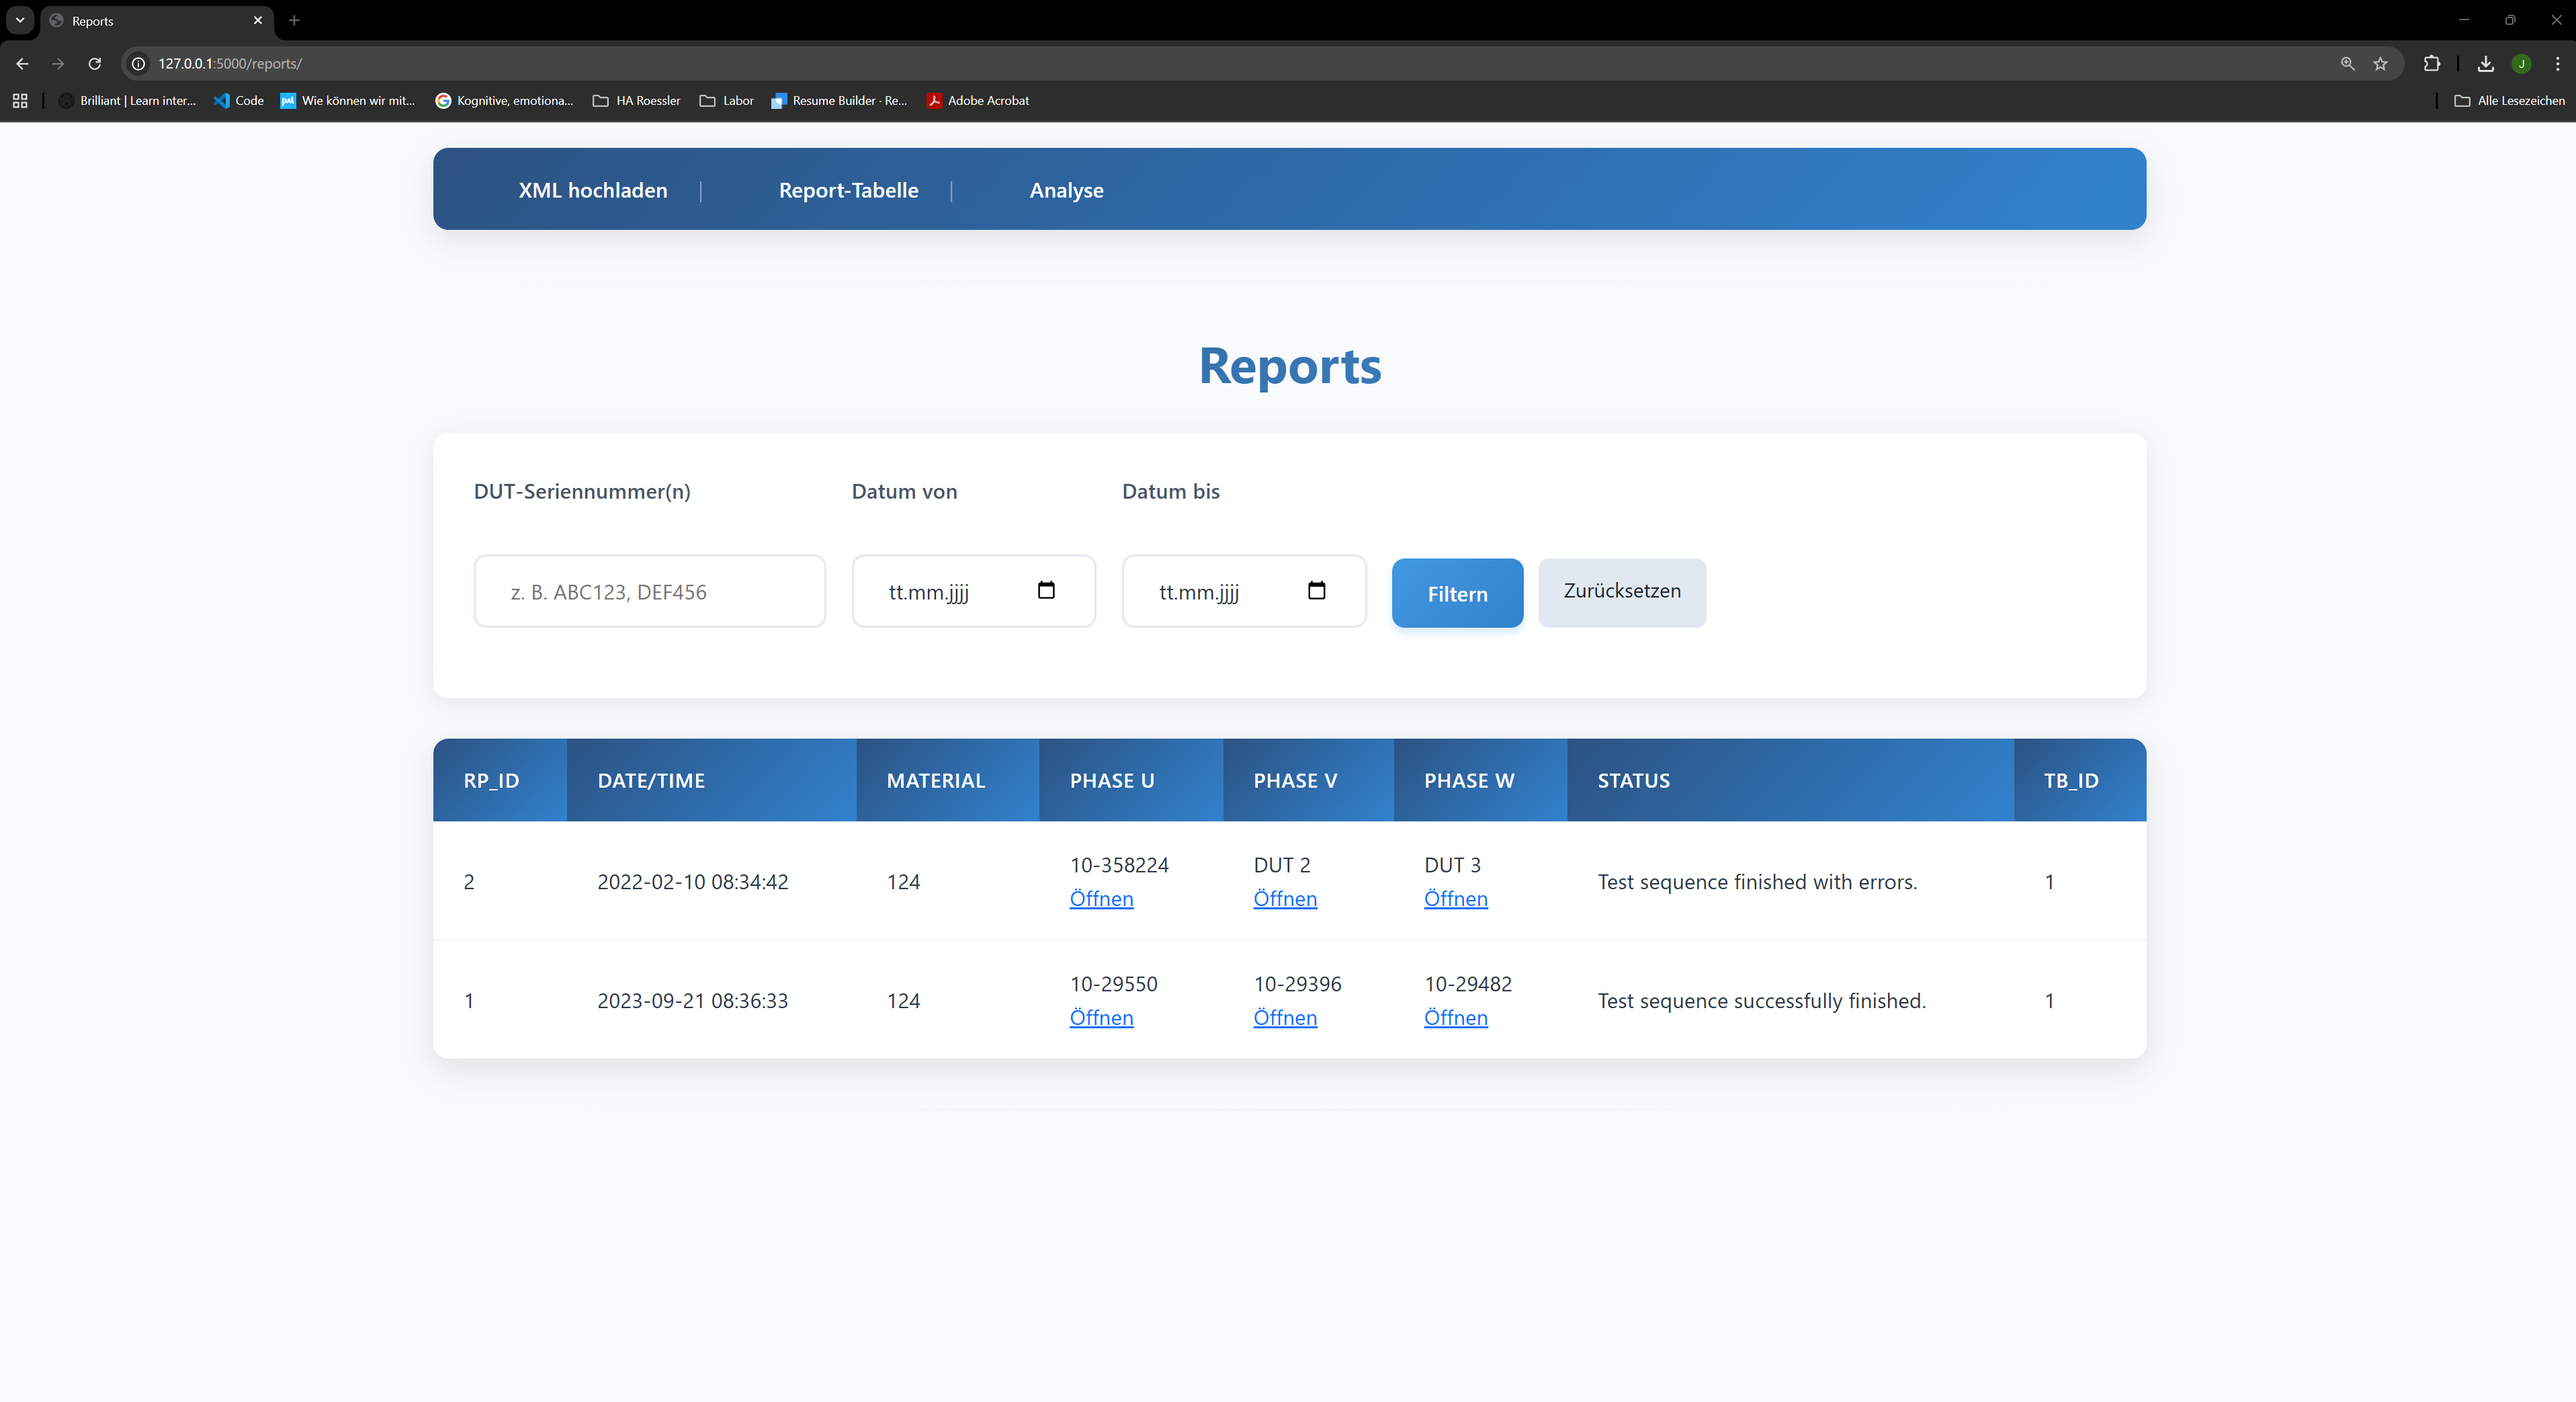
\includegraphics[width=1\textwidth]{Grafiken/Bild Reports}
    \caption{Erstellte Webseite für Report-Tabelle in Browserfenster}
    \label{fig: Webseite für Report-Tabelle}
    {Quelle: Eigene Darstellung}
\end{figure}

3. Analyse (\code{dut\_analyse.html}): Darstellung ausgewählter Messdaten eines DUT aus einem Testbericht in grafischer Form.
Die Seite ist in der folgenden Abbildung \ref{fig: Webseite für Analyse} dargestellt.

\begin{figure}[H]
    \centering
    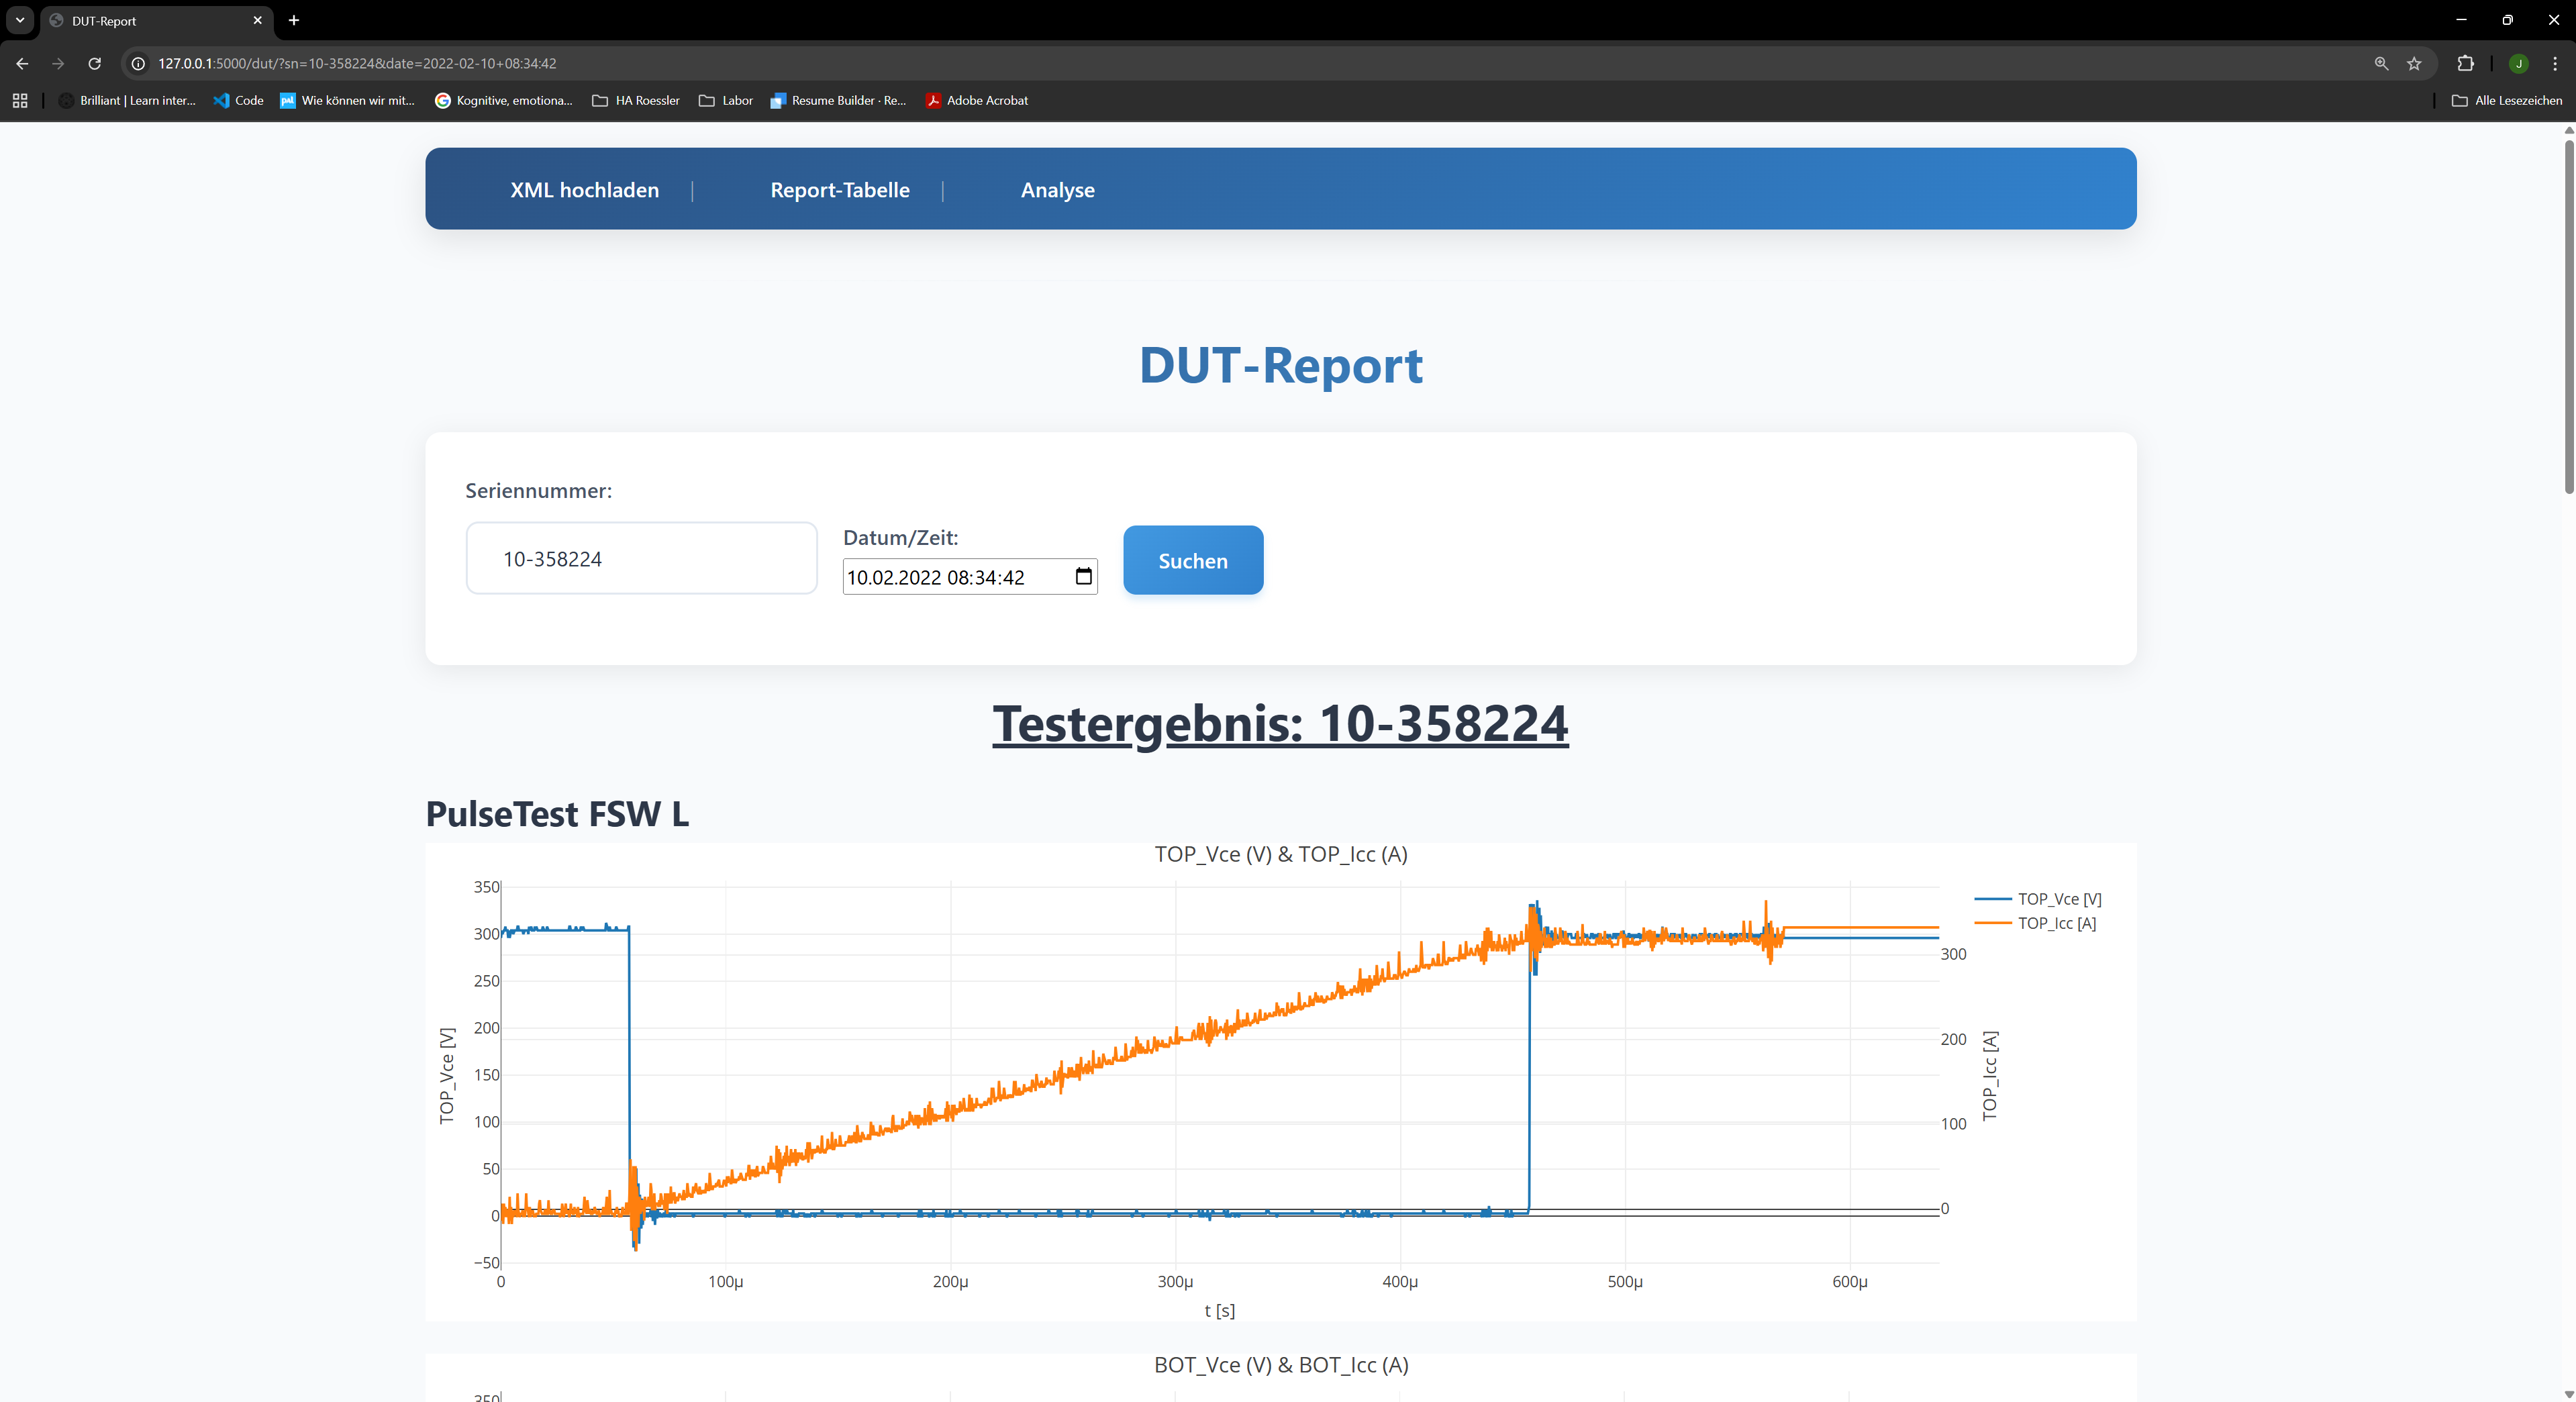
\includegraphics[width=1\textwidth]{Grafiken/Bild DUT-Report}
    \caption{Erstellte Webseite für Analyse in Browserfenster}
    \label{fig: Webseite für Analyse}
    {Quelle: Eigene Darstellung}
\end{figure}


Im Folgenden wird anhand der Beschreibung des
Jinja2-Templates (\code{upload.html}) erläutert, wie die Übermittlung der Daten
über einen Buttondruck an die Logikschicht abläuft. Dieses Prinzip wird in
allen Jinja2-Templates benutzt, um eingegebene Daten aus den Eingabefeldern der
Webseite an die Logikschicht zu übermitteln.


Der Code aus \code{upload.html} ist in der Abbildung \ref{fig: Programmcode aus upload.html} für ein besseres Verständnis dargestellt.

\begin{figure}[H]
    \centering
    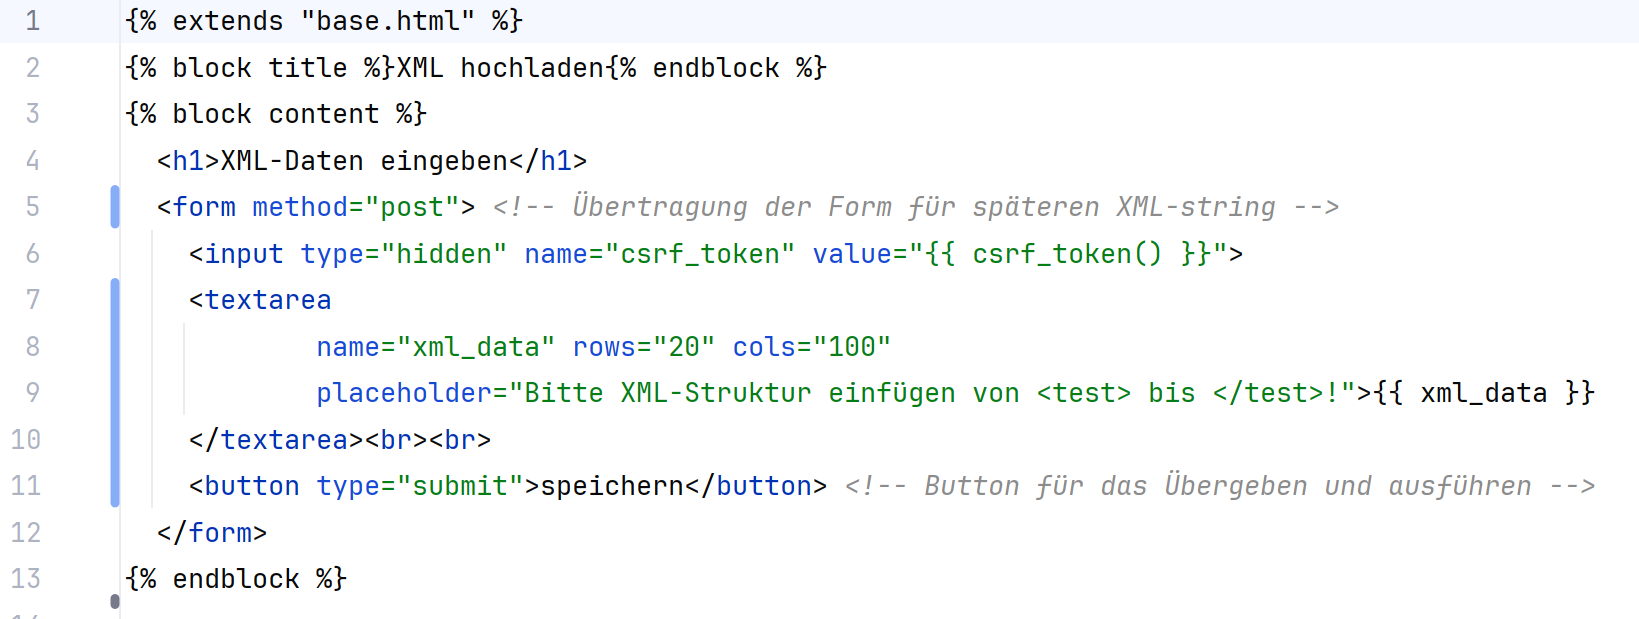
\includegraphics[width=1\textwidth]{Grafiken/Beispiel Programmcode aus upload.html}
    \caption{Beispiel Programmcode aus upload.html}
    \label{fig: Programmcode aus upload.html}
    {Quelle: eigene Darstellung}
\end{figure}

Wie bereits oben schon genannt, erweitert das Template \code{upload.html} die
in \code{base.html} definierte Grundstruktur und fügt deren allgemeine Elemente
wie Navigationsleiste, Kopfbereich und Mitteilungsfeld ein. Innerhalb des „blocks
content“ wird der seitenindividuelle Inhalt definiert. Hierzu gehört ein
Eingabefeld in Form eines HTML-Formulars, das zur Eingabe der XML-Struktur
dient.

Das Formular verwendet die Methode „POST“, wodurch die
eingegebenen Daten an die Serverlogik gesendet werden, sobald der Benutzer den
Button \textit{„speichern“} betätigt. Über das „csrf\_token“-Feld wird ein
Sicherheitsmechanismus implementiert, der Cross-Site-Request-Forgery-Angriffe
verhindert. Der eigentliche Eingabebereich wird durch ein „<textarea>“-Element
realisiert, das genügend Platz bietet, um den XML-Inhalt beginnend mit dem
Stammelement „<test>“ bis zum schließenden „</test>“ vollständig
einzufügen.

Beim Betätigen des Buttons wird der Inhalt des Textfeldes an
die zugehörige Flask-Route, in diesem Fall \code{routes.py} im Unterordner \code{upload}
in \code{blueprints} übergeben, wo die Daten serverseitig verarbeitet werden.
Die Applikationslogik übernimmt in diesem Fall anschließend das Einlesen, Validieren und Speichern der XML-Struktur in der Datenbank.

Dieses Prinzip findet sich in gleicher Form auch in den
anderen Templates für die Filterfunktionen der Applikation wieder, wodurch eine einheitliche und
konsistente Interaktion zwischen Benutzeroberfläche und Logikschicht
gewährleistet wird.



























